\documentclass[11pt]{article}

% Handle Spanish seamlessly!
\usepackage[utf8]{inputenc}
\usepackage[spanish, es-tabla]{babel}

% Change the language for the captions and default names
\renewcommand{\figurename}{Figura}

% Needed for the multline environment
\usepackage{amsmath}

% Images
\usepackage{graphicx}
\graphicspath{{Img/}}

\usepackage{geometry}
\geometry{
    a4paper,
    left = 20mm,
    right = 20mm,
    top = 15mm,
    bottom = 15mm
}

\title{Acostumbrándonos al entorno \texttt{GNS3}}
\author{Pablo Collado Soto \\ \\ \textit{Ingeniería de Tráfico}}
\date{}

\begin{document}
    \maketitle

    \section{Introducción}
        En esta práctica vamos a intentar familiarizarnos con el entorno \texttt{GNS3} así como con \texttt{mgen}, herramienta con la que generamos tráfico para poner a prueba la red bajo estudio. Tenga en cuenta que los archivos que se han empleado para generar tráfico en el escenario, así como los archivos que recogen el tráfico real sobre la red se adjuntan en el repositorio asociado.\\

        En nuestro escenario contamos con un equipo \texttt{SRC} que generará tráfico que atravesará al router \texttt{R1} para llegar al equipo \texttt{DST}. Como cabría esperar, \texttt{R1} cuenta con $2$ interfaces. La primera pertenece a la misma subred que \texttt{SRC} y la segunda a la misma que \texttt{DST}. Para poder controlar la congestión en el encaminador a nuestro antojo modificaremos la velocidad de la interfaz conectada a \texttt{DST} desde el punto de vista de la capa de red. Al estar empleando interfaces \texttt{fastEthernet} podríamos esperar una tasa en las líneas asociadas de $100\ Mbps$. No obstante y debido a las limitaciones intrínsecas a nuestro escenario virtualizado veremos que esas velocidades se ``quedan'' en unos $20\ Mbps$. No especificamos una velocidad ya que la velocidad real variará ligeramente en función de la potencia del equipo sobre el que ejecutemos las simulaciones. En nuestro caso disponemos de $16\ GB$ de memoria \texttt{RAM} y un procesador \textit{Intel(R) Core(TM) i7-5500U CPU @ 2.40GHz} tal y como indica el comando \texttt{lscpu}. Nuestro sistema operativo anfitrión es \texttt{Ubuntu 20.04}.

        \subsection{Configurando carpetas compartidas}
            Antes de proceder a probar el escenario queremos dedicar una pequeña sección a explicar la configuración que hemos llevado a cabo en las máquinas virtuales para poder extraer los archivos que recogen las trazas de tráfico en base a las cuales obtendremos las gráficas que adjuntamos en el documento. Personalmente no nos agrada demasiado trabajar dentro de máquinas virtuales y, al estar ejecutando \texttt{Ubuntu} de forma nativa preferimos generar las gráficas en nuestro propio equipo para poder guardarlas de manera más cómoda.\\

            Para conseguir compartir archivos basta con configurar las carpetas compartidas en cada una de las $3$ máquinas virtuales del entorno. Comenzaremos explicando la jerarquía que debemos crear desde la máquina anfitriona. En el sistema operativo nativo solo debemos crear un directorio en el que se almacenarán todos los archivos generados. En nuestro caso lo hemos nombrado \texttt{VMWare\_shares} y la ruta absoluta hasta él viene dada por \texttt{/home/pablo/VMWare\_shares}. En el \textit{VMWare Player} que ejecutamos en el anfitrión configuraremos una carpeta compartida en el menú \texttt{Virtual Machine > Virtual Machine Settings} al que también podemos acceder con \texttt{CTRL + D}. Una vez dentro hacemos click en \texttt{Options} y creamos una carpeta compartida cuyo \texttt{Host Path} apunte a \texttt{/home/pablo/VMWare\_shares}. Debemos anotar el nombre que le damos al directorio compartido ya que después de crearlo aparecerá la carpeta \texttt{/mnt/hgfs/Foo} donde \texttt{Foo} es el nombre que nosotros le hemos dado a la carpeta compartida en cuestión. A fin de trabajar de manera más cómoda hemos creado un \textit{enalce simbólico} a dicho directorio en el directorio de conexión del usuario \texttt{itraf} en la máquina virtual. En otras palabras, hemos ejecutado \texttt{ln -s /mnt/hgfs/Foo /home/itraf/Host\_shares} con lo que el directorio \texttt{Host\_shares} es un enlace a la carpeta compartida.\\

            En cada una de las máquinas que lanzamos al ejecutar el escenario de \texttt{GNS3} haremos algo parecido. Navegando por \texttt{VM > Settings} (o pulsando de nuevo \texttt{CTRL + D}) configuramos una nueva carpeta compartida en cada máquina. Llamaremos a dicha carpeta \texttt{Foo} de nuevo y la apuntaremos contra el directorio \texttt{/home/itraf/Host\_shares} de la máquina virtual "original". Para trabajar de forma más cómoda ejecutaremos \texttt{ln -s /mnt/hgfs/Foo /home/itraf/Int\_shares} en cada máquina del escenario de \texttt{GNS3} para lograr lo mismo que hacíamos con el directorio \texttt{Host\_shares} en el párrafo anterior.\\

            Tal y como está montado el escenario ahora basta con mover un archivo a la carpeta \texttt{Int\_shares} en cualquiera de las máquinas lanzadas por \texttt{GNS3} para que éste aparezca en la carpeta \texttt{VMWare\_shares} del sistema operativo anterior. Así podemos extraer los archivos necesarios de una manera sencilla para procesarlos más tarde sin tener la monstruosidad de escenario devorando memoria \texttt{RAM} como si no hubiera un mañana.

    \section{Generando tráfico sin saturar el router}
        En una primera instancia intentaremos generar tráfico sin saturar el enlace de salida del router a fin de no provocar que el \textit{buffer} de salida del router se desborde. Para ello debemos recordar que la interfaz de salida del mismo tiene una tasa de alrededor de $20\ Mbps$. Tal y como sugiere el guión de la práctica vamos a configurar \texttt{SRC} para que emita $4$ flujos de datos de tal manera que en el momento de mayor solapamiento solo tengamos una tasa de entrada total de $17\ Mbps$. Para controlar el ``caudal'' de cada flujo podemos alterar el tamaño del paquete en la capa de aplicación (esto es, la \textit{SDU} de la capa de transporte) o el número de paquetes de ese tamaño que la capa de aplicación emite por segundo. Dado que ambos parámetros controlan de manera directa el ``tamaño'' de los flujos fijaremos uno de ellos para variar el otro hasta conseguir el objetivo deseado.\\

        Las velocidades de los flujos vienen dadas por:

        \begin{center}
            \begin{tabular}{|c|c|c|c|}
                \hline
                & \texttt{Instante de comienzo [s]} & \texttt{Instante de fin [s]} & \texttt{Tasa [Mbps]}\\
                \hline
                1 & 0 & 20 & 8\\
                \hline
                2 & 5 & 20 & 1\\
                \hline
                3 & 10 & 20 & 4\\
                \hline
                4 & 15 & 20 & 4\\
                \hline
            \end{tabular}
        \end{center}

        En nuestro caso vamos a fijar el tamaño de la \textit{SDU} en la capa de transporte a $1250\ B$. Aún añadiendo las cabeceras de \texttt{UDP, IP} y \texttt{Ethernet} tenemos un tamaño total en la capa física de $L_{phys} = 1250 + 8 + 20 + 38 = 1316\ B$. Recordemos que la \textit{MTU} típica de \texttt{Ethernet} es de $1500\ B$ con lo que no la estamos superando. De hacerlo deberíamos tener en cuenta el aumento de sobrecarga de cabeceras al que nos enfrentaríamos ya que un mensaje de la capa de aplicación requeriría más de una trama en la capa de enlace.\\

        Si comparamos la sobrecarga introducida por las cabeceras con el tamaño del mensaje veremos que éstas no representan ni siquiera el $5,3\%$ del total del paquete ($\frac{L_{hdr}}{L_{app}} = \frac{8 + 20 + 38}{1250} = 0,0528 < 0,053$). Esto implica que la velocidad en la capa física ($V_{phy}$) será un $5,3\%$ mayor que la de la capa de aplicación ($V_{app}$), que es la que vamos a medir.

        $$\frac{V_{phy}}{V_{app}} = \frac{\frac{L_{phy}}{t}}{\frac{L_{app}}{t}} = \frac{L_{phy}}{L_{app}} = \frac{L_{app} + L_{hdr}}{L_{app}} = 1 + \frac{66\ B}{1250\ B} = 1 + 0,0528 \rightarrow V_{phy} = 1,0528 \cdot V_{app}$$

        Despreciaremos esta diferencia pero es bueno conocer que existe tal y como nos invita a hacer el guión de la práctica.\\

        En cualquier caso con un tamaño de mensaje $L_{app} = 1250\ B$ estamos dentro de los límites de la \textit{MTU} de \texttt{Ethernet} con lo que es apropiado. Una vez decidido esto vamos a ver cómo podemos lograr una velocidad determinada en un flujo variando el número de mensajes por segundo $N$. Aplicando la mismísima definición de tasa en la ecuación \ref{eq:1} llegamos a una expresión que nos permite controlar la tasa de cada flujo.

        \begin{multline} \label{eq:1}
            V_e = N\ \frac{pkt}{s}\ \cdot 1250\ \frac{B}{pkt}\ \cdot 8\ \frac{b}{B} \rightarrow V_e = N \cdot 10^4\ bps \rightarrow N = 10^{-4} \cdot V_e\ [bps] \rightarrow\\
            \rightarrow N = 10^{-4} \cdot V_e \cdot 10^6\ \frac{Mbps}{bps} = 100 \cdot V_e\ [Mbps]
        \end{multline}

        Esto es, que si queremos un flujo de $8\ Mbps$ debemos especificar $N = 100 \cdot 8 = 800\ \frac{pkt}{s}$ en la configuración de \texttt{mgen} en el emisor. Así, los parámetros de configuración de cada flujo se recogen en la tabla \ref{tab:conf}. Teniendo esto claro vamos a adjuntar cada una de las figuras (figuras \ref{fig:nomR}-\ref{fig:nomLoss}) que se nos requerían en este caso.

        \begin{table}
            \centering
            \begin{tabular}{|c|c|c|}
                \hline
                & \texttt{Paquetes por segundo} & \texttt{Tamaño de la SDU de UDP [B]}\\
                \hline
                1 & 800 & 1250\\
                \hline
                2 & 100 & 1250\\
                \hline
                3 & 400 & 1250\\
                \hline
                4 & 400 & 1250\\
                \hline
            \end{tabular}
            \caption{Configuración de los flujos}
            \label{tab:conf}
        \end{table}

        \begin{figure}
            \centering
            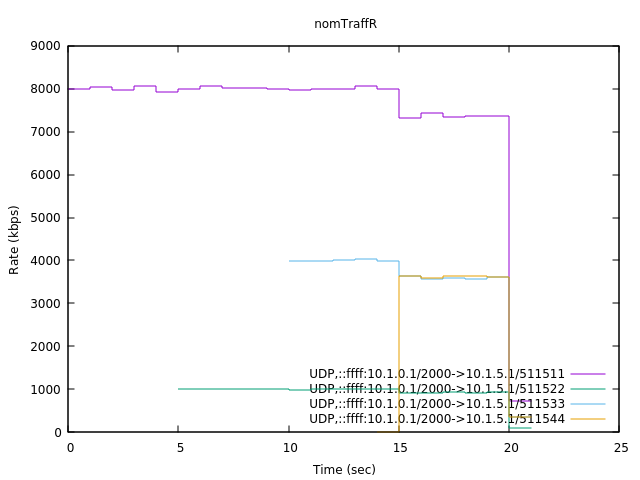
\includegraphics[width=0.6\linewidth]{nomTraffR.png}
            \caption{Tasa de cada flujo.}
            \label{fig:nomR}
        \end{figure}

        \begin{figure}
            \centering
            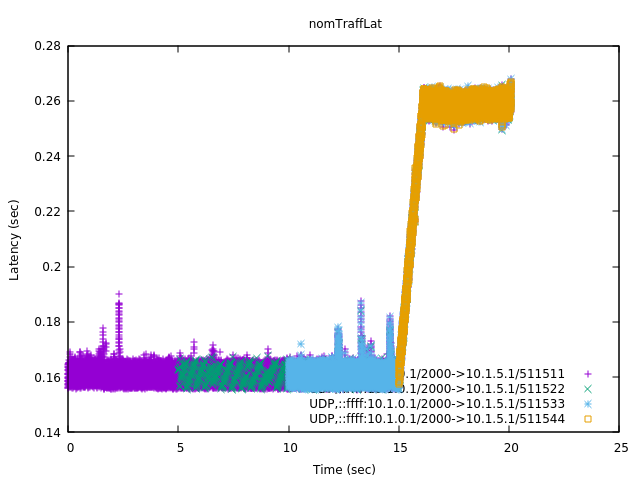
\includegraphics[width=0.6\linewidth]{nomTraffLat.png}
            \caption{Latencia de cada flujo.}
            \label{fig:nomLat}
        \end{figure}

        \begin{figure}
            \centering
            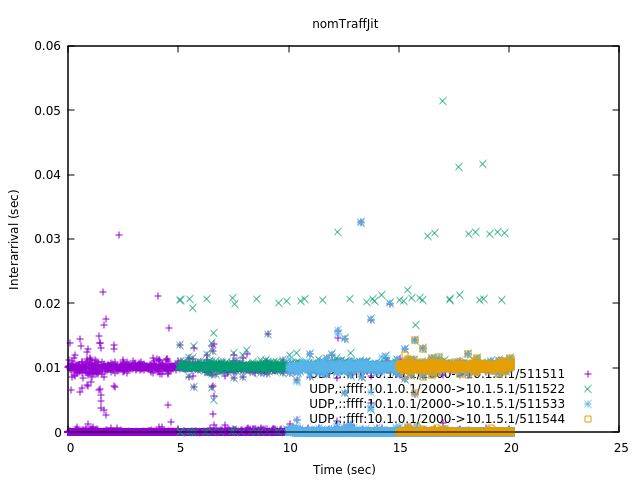
\includegraphics[width=0.6\linewidth]{nomTraffJit.png}
            \caption{\textit{Jitter} de cada flujo.}
            \label{fig:nomJit}
        \end{figure}

        \begin{figure}
            \centering
            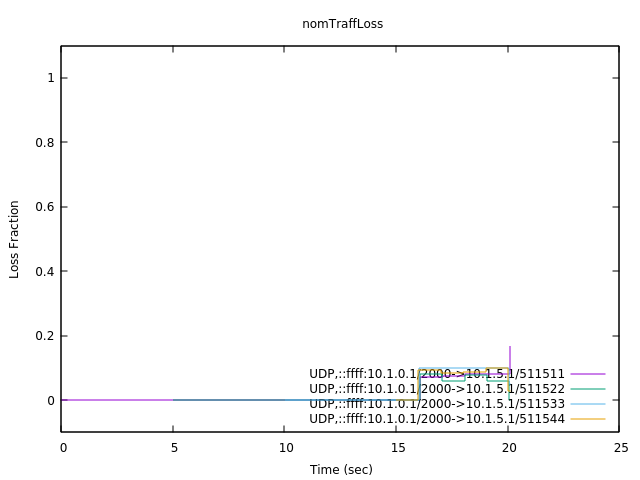
\includegraphics[width=0.6\linewidth]{nomTraffLoss.png}
            \caption{Pérdidas de cada flujo.}
            \label{fig:nomLoss}
        \end{figure}

        \subsection{Comentando las gráficas \ref{fig:nomR}-\ref{fig:nomLoss}}
            Observando las gráficas vemos que, aunque no debería estar ocurriendo, el buffer de \texttt{R1} se está saturando. La latencia comienza a crecer cuando tenemos un flujo acumulado de $17\ Mbps$ hasta saturar pocos instantes después de $15\ s$. De ésto deducimos que la velocidad real de la interfaz de salida de \texttt{R1} en nuestro equipo es menor de $17\ Mbps$. Asociada a esta saturación del buffer tras $t = 15\ s$ tenemos una pérdida de paquetes. El \textit{jitter} es prácticamente constante pero deberíamos observar un pequeño pico en el momento en el que el buffer se empieza a saturar.

            Debido a que estos resultados no son los que esperaríamos decidimos repetir la prueba con flujos de menor tasa para observar las gráficas que se generarían en una situación sin congestión. Las incluimos en la siguiente sección.

    \section{Rebajando el tráfico para evitar saturar el router}
        A fin de evitar la saturación del encaminador hemos decidido rebajar la tasa de los flujos para que quede tal y como se recoge en la tabla \ref{tab:low_conf}.

        \begin{table}
            \centering
            \begin{tabular}{|c|c|c|c|}
                \hline
                & \texttt{Instante de comienzo [s]} & \texttt{Instante de fin [s]} & \texttt{Tasa [Mbps]}\\
                \hline
                1 & 0 & 20 & 4\\
                \hline
                2 & 5 & 20 & 1\\
                \hline
                3 & 10 & 20 & 4\\
                \hline
                4 & 15 & 20 & 4\\
                \hline
            \end{tabular}
            \caption{Rebajando la tasa del flujo 1.}
            \label{tab:low_conf}
        \end{table}

        Con la nueva configuración de la tabla \ref{tab:low_conf} generamos las figuras \ref{fig:lowR}-\ref{fig:lowLoss}.

        \begin{figure}
            \centering
            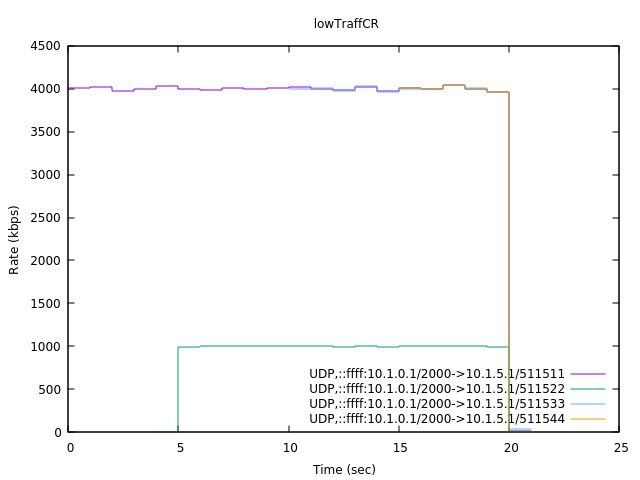
\includegraphics[width=0.6\linewidth]{lowTraffR.png}
            \caption{Tasa de cada flujo.}
            \label{fig:lowR}
        \end{figure}

        \begin{figure}
            \centering
            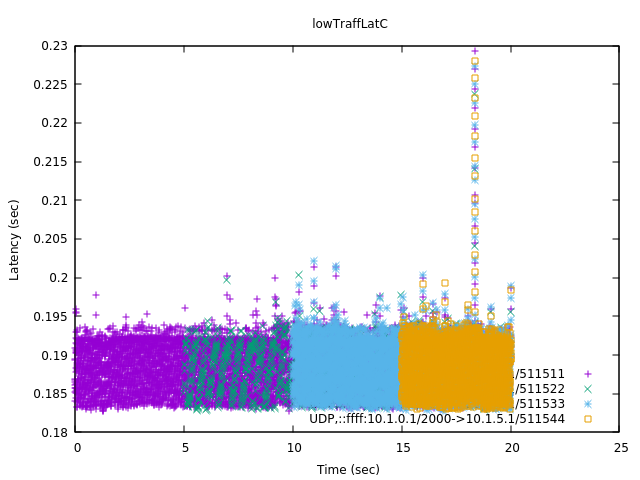
\includegraphics[width=0.6\linewidth]{lowTraffLat.png}
            \caption{Latencia de cada flujo.}
            \label{fig:lowLat}
        \end{figure}

        \begin{figure}
            \centering
            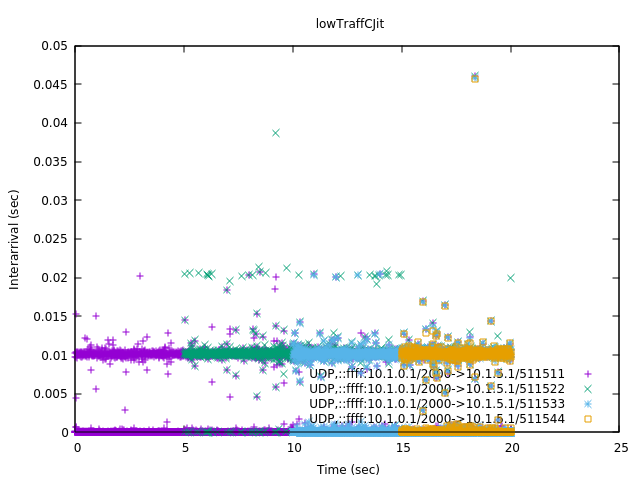
\includegraphics[width=0.6\linewidth]{lowTraffJit.png}
            \caption{\textit{Jitter} de cada flujo.}
            \label{fig:lowJit}
        \end{figure}

        \begin{figure}
            \centering
            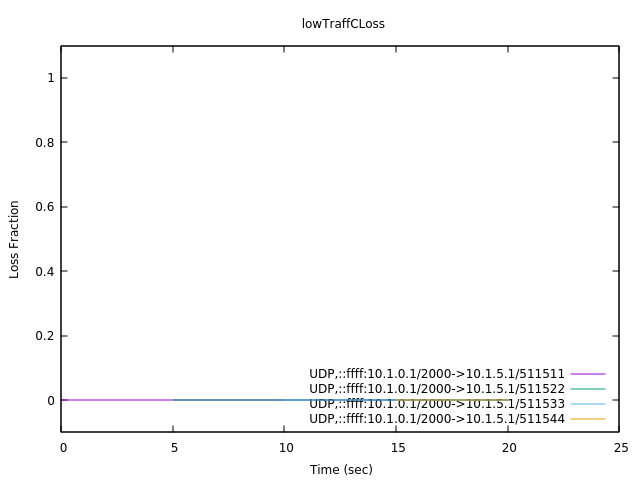
\includegraphics[width=0.6\linewidth]{lowTraffLoss.png}
            \caption{Pérdidas de cada flujo.}
            \label{fig:lowLoss}
        \end{figure}

        \subsection{Comentando las gráficas \ref{fig:lowR}-\ref{fig:lowLoss}}
            Observamos que la pérdida es nula para cada uno de los flujos y que la latencia es prácticamente constante en el periodo de $20\ s$ que dura la prueba. Con lo que el buffer no llega a llenarse. De esto deducimos que la tasa real de la interfaz de salida es mayor que $13\ Mbps$, el total máximo que experimentamos durante la prueba. También debemos comentar que el \textit{jitter} es prácticamente constante ya que la latencia también lo es.

    \section{Limitando la interfaz de salida a $10\ Mbps$}
        Tal y como comenta el guión configuramos \texttt{R1} para que limite la velocidad de la interfaz de salida a $10\ Mbps$. Recuperando la configuración inicial de los flujos llegamos a las gráficas que se recogen en las figuras \ref{fig:congR}-\ref{fig:congLoss}.

        \begin{figure}
            \centering
            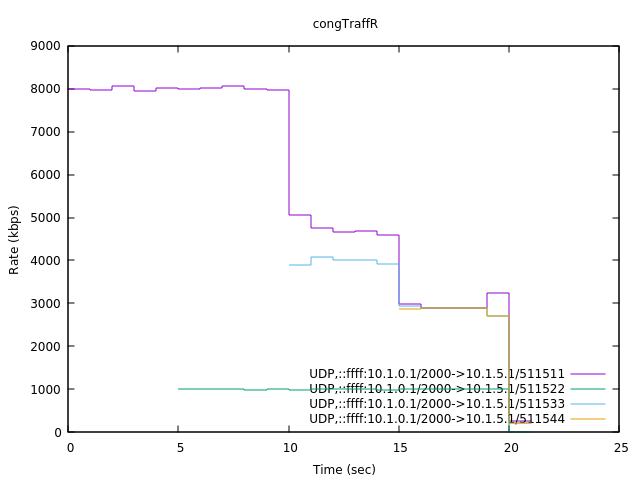
\includegraphics[width=0.6\linewidth]{congTraffR.png}
            \caption{Tasa de cada flujo.}
            \label{fig:congR}
        \end{figure}

        \begin{figure}
            \centering
            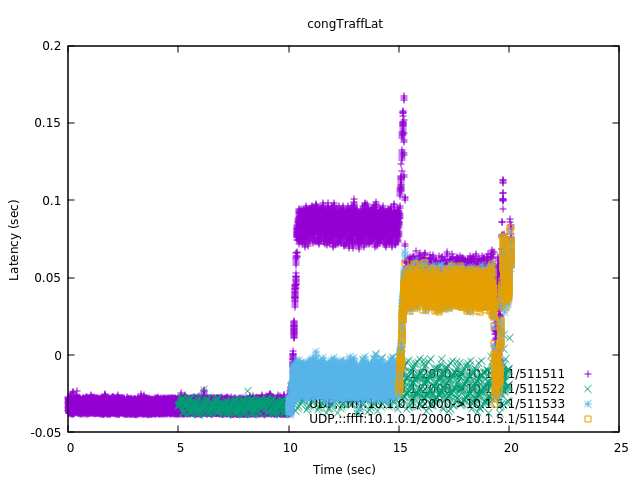
\includegraphics[width=0.6\linewidth]{congTraffLat.png}
            \caption{Latencia de cada flujo.}
            \label{fig:congLat}
        \end{figure}

        \begin{figure}
            \centering
            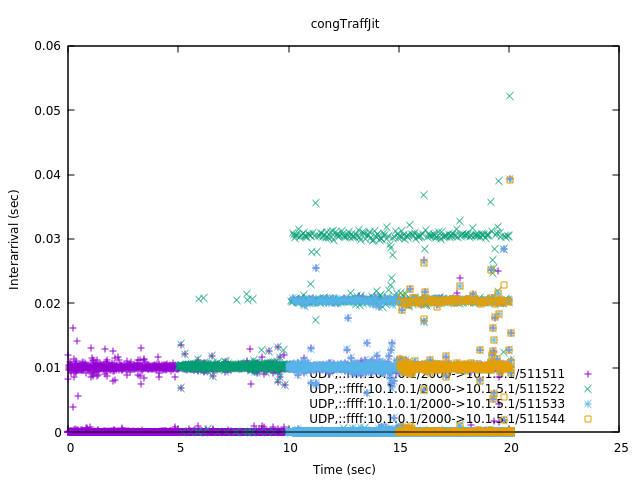
\includegraphics[width=0.6\linewidth]{congTraffJit.png}
            \caption{\textit{Jitter} de cada flujo.}
            \label{fig:congJit}
        \end{figure}

        \begin{figure}
            \centering
            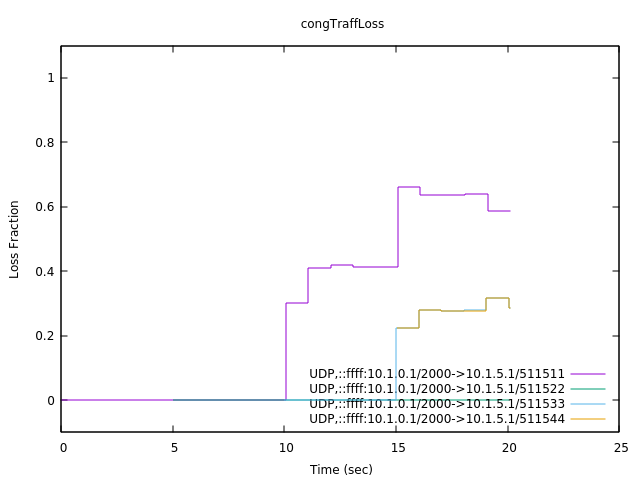
\includegraphics[width=0.6\linewidth]{congTraffLoss.png}
            \caption{Pérdidas de cada flujo.}
            \label{fig:congLoss}
        \end{figure}

        \subsection{Comentando las gráficas \ref{fig:congR}-\ref{fig:congLoss}}
            Antes de llevar a cabo las pruebas esperábamos observar una gráfica de latencia parecida a la que obtuvimos en la figura \ref{fig:nomLat}. No obstante generamos la gráfica de la figura \ref{fig:congLat}. Se aprecia que la latencia comienza a subir cuando se incorporan más flujos a la prueba pero no llegamos a saturar el buffer como lo hacíamos en el primer escenario. Dada la variabilidad del escenario desconocemos qué está provocando este comportamiento pero sí observamos una diferencia tras alterar la configuración de \texttt{R1}. Sí que provocamos una pérdida de paquetes tal y como vemos en la figura \ref{fig:congLoss} que se produce cuando la tasa agregada de los flujos es mayor que la velocidad de la interfaz de salida. Ésto se sigue del hecho de que en ausencia de mecanismos \textit{QoS} el buffer del router es una simple cola \textit{FIFO}. Veamos cómo se compota el buffer para cada uno de los tramos de la prueba.

            \subsubsection{Tramo 1: $t \in [0,\ 5]\ s$}
                En este caso solo tenemos un flujo de $8\ Mbps$ con lo que su tasa de salida será la misma ya que es menor que la velocidad de la interfaz: $10\ Mbps$.

            \subsubsection{Tramo 2: $t \in [5,\ 10]\ s$}
                Al igual que antes, solo tendremos $2$ flujos con una tasa agregada de $9\ Mbps$ que sigue siendo menor que la tasa de la interfaz de salida. Cada flujo tendrá una tasa de salida igual que la de entrada.

            \subsubsection{Tramo 3: $t \in [10,\ 15]\ s$}
                En este tramo ya tenemos una tasa agregada de $13\ Mbps$ con lo que se producirá un reparto proporcional:

                \begin{align*}
                    V_{o_x} &= \frac{V_{i_x}}{\sum_{x = 1}^3 V_{i_x}} \cdot V_o\\
                    V_{o_1} &= \frac{8\ Mbps}{8\ Mbps + 1\ Mbps + 4\ Mbps} \cdot 10\ Mbps \approx 6,154\ Mbps\\
                    V_{o_2} &= \frac{1\ Mbps}{8\ Mbps + 1\ Mbps + 4\ Mbps} \cdot 10\ Mbps \approx 0,769\ Mbps\\
                    V_{o_3} &= \frac{4\ Mbps}{8\ Mbps + 1\ Mbps + 4\ Mbps} \cdot 10\ Mbps \approx 3,077\ Mbps
                \end{align*}

            \subsubsection{Tramo 4: $t \in [15,\ 20]\ s$}
                Tan solo debemos añadir un flujo al procedimiento anterior:

                \begin{align*}
                    V_{o_x} &= \frac{V_{i_x}}{\sum_{x = 1}^4 V_{i_x}} \cdot V_o\\
                    V_{o_1} &= \frac{8\ Mbps}{8\ Mbps + 1\ Mbps + 4\ Mbps + 4\ Mbps} \cdot 10\ Mbps \approx 4,706\ Mbps\\
                    V_{o_2} &= \frac{1\ Mbps}{8\ Mbps + 1\ Mbps + 4\ Mbps + 4\ Mbps} \cdot 10\ Mbps \approx 0,588\ Mbps\\
                    V_{o_3} &= \frac{4\ Mbps}{8\ Mbps + 1\ Mbps + 4\ Mbps + 4\ Mbps} \cdot 10\ Mbps \approx 2,353\ Mbps\\
                    V_{o_4} &= \frac{4\ Mbps}{8\ Mbps + 1\ Mbps + 4\ Mbps + 4\ Mbps} \cdot 10\ Mbps \approx 2,353\ Mbps
                \end{align*}

    \section{Conclusión}
        En definitiva, vemos cómo y por qué se manifiesta la congestión en un encaminador y nos damos cuenta de la necesidad de procedimientos \textit{QoS} para poder priorizar según y qué flujos en función de las necesidades del servicio requerido. En la siguiente práctica asistiremos a la configuración de mecanismos \textit{QoS}.
\end{document}
